\subsection{Spearman}
Spearman formulò questa misura statistica per permettere il calcolo delle relazioni di tipo non lineare tra due variabili. I criteri che permettono di sfruttare questo coefficiente si fermano ai primi due step dell'indice di Pearson, il coefficiente di Spearman si può infatti definire come un caso specifico di indice di Pearson che trasforma i dati in ranghi prima di calcolare il coefficiente. 
\[\rho _{s}={\frac {\sum _{i}(r_{i}-{\overline {r}})(s_{i}-{\overline {s}})}{{\sqrt {\sum _{i}(r_{i}-{\overline {r}})^{2}}}{\sqrt {\sum _{i}(s_{i}-{\overline {s}})^{2}}}}}\]
In applicazioni pratiche si utilizza una formula semplificata: \(\rho _{s}=1-{\frac {6\sum _{i}D_{i}^{2}}{N(N^{2}-1)}}\) dove \(D_i\) rappresenta la differenza tra i ranghi \(r_{i}-s_{i}\) delle due variabili confrontate. \\
Per verificare l'ipotesi appena citata viene comparato il risultato con la variabile casuale di Spearman, per casi in cui \(N > 20\) invece si fa ricorso alla variabile t di Student. 
\[t = \rho_S ({\frac{1-\rho_S^2}{n-2}})^{-\frac{1}{2}}\]
L'interpretazione di questo coefficiente è data da una relazione di dipendenza della variabile Y dalla variabile X indipendente, per questo motivo più si avvicina a 1 il valore di Spearman e più la correlazione sarà forte.
\subsubsection{Applicazione}
\begin{tabular}{ ||p{2cm}|p{2cm}|p{2cm}|p{2cm}|p{2cm}|p{2cm}||  }
 \hline
 Nationality & Destination & Crunchbase & ESTAT & ri & si\\ [0.5ex] 
 \hline\hline\hline
 ROU& ITA& 10& 234& 6& 1\\
 \hline
 ROU& AUS& 23& 222& 4& 2\\
 \hline
 AUS& ITA& 55& 33& 1& 5\\
 \hline
 AUS& AUS& 33& 120& 3& 4\\
 \hline
 GBR& USA& 11& 14& 5& 6\\
 \hline
 GBR& USA& 43& 123& 2& 3\\
 \hline
\end{tabular}
\paragraph{Pearson}
\[^\rho{XY}  = \frac{^\sigma{XY}}{^\sigma{X} ^\sigma{Y}} = \]
\[^\sigma{XY}  = -618,86\]
\[^\sigma{X} = \sqrt{\frac{1}{6}*[110^2+98^2+(-91)^2+(-4)^2+(-110)^2+(-1)^2]} = \sqrt{\frac{42102}{6}} = 83,76\]
\[^\sigma{Y} = \sqrt{\frac{1}{6}*[(-19)^2+(-6)^2+26^2+4^2+(-18)^2+14^2]} = \sqrt{\frac{1}{6}} = 16,37\]
\[^\rho{XY} = \frac{-618,86}{16,37*83,76} = -0,45\]
\paragraph{Spearman}
\[\rho _{s}=1-{\frac {6\sum _{i}D_{i}^{2}}{N(N^{2}-1)}} =\]
\[1 - \frac{\cancel{6}*[(6-4)^2+(4-2)^2+(1-5)^2+(3-4)^2+(5-6)^2+(2-3)^2]}{\cancel{6}(6^2-1)=35} =\]
\[1 - \frac{4+4+16+1+1+1}{35} = 1 - \frac{27}{35} = 0.22\]
Questo esempio non è da considerarsi reale, in quanto sono stati usati dati fittizi solo per rendere chiaro il concetto di rango, ovvero l'indice di posizione del numero nell'insieme ordinato.






%%%%% CITTADINI CONFRONTO ESTAT 
\begin{figure}[t]
    \centering
    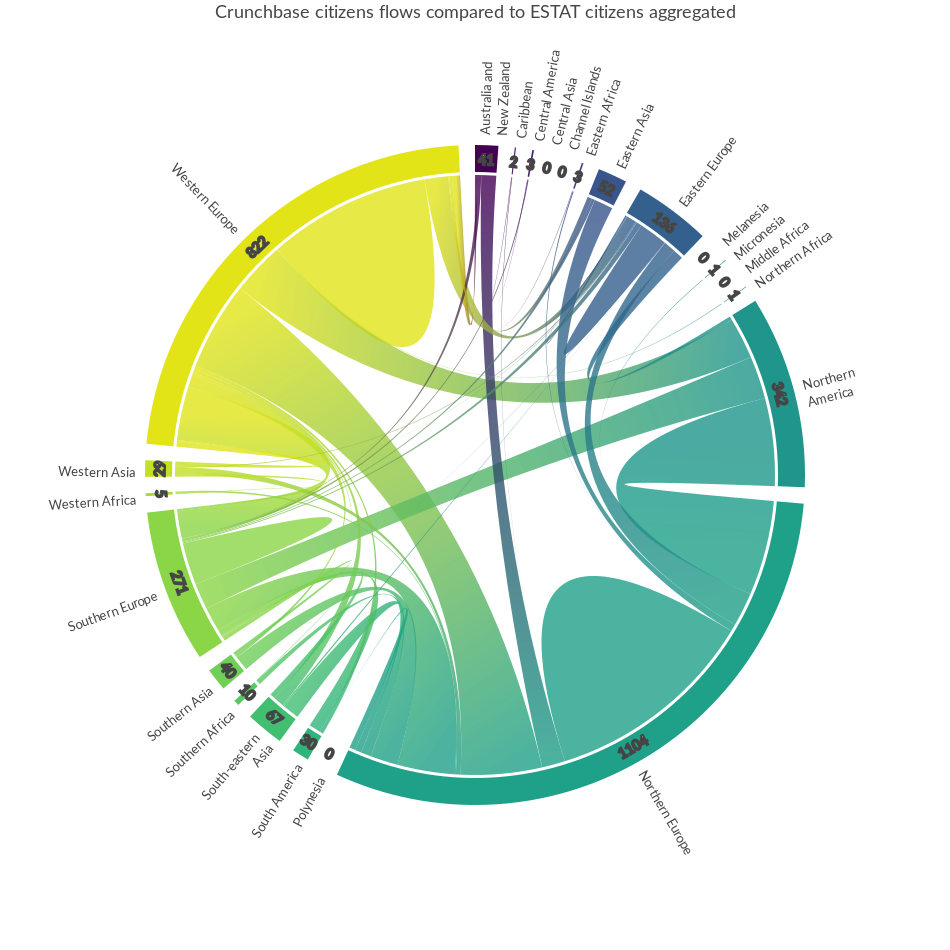
\includegraphics[width=1.0\textwidth]{images/ChordFlows/Crunchbase_cit_ESTAT_True.png}
    \caption{Chordflow flussi Crunchbase in comparazione ai cittadini ESTAT}
    \label{fig:chordcrunchestatcittrue}
\end{figure}
Questo grafico che %analizza
mostra i flussi dei cittadini su Crunchbase, oltre ad essere più accattivante a livello grafico, permette di vedere una gran parte di flussi rientranti nella stessa zona. Per compararne i risultati, %possiamo vedere di seguito 
la Figura \ref{fig:chordestatcittrue} %che analizza 
mostra i flussi migratori dei cittadini %attraverso 
in ESTAT per vari sub-continenti. 
\begin{figure}[t]
    \centering
    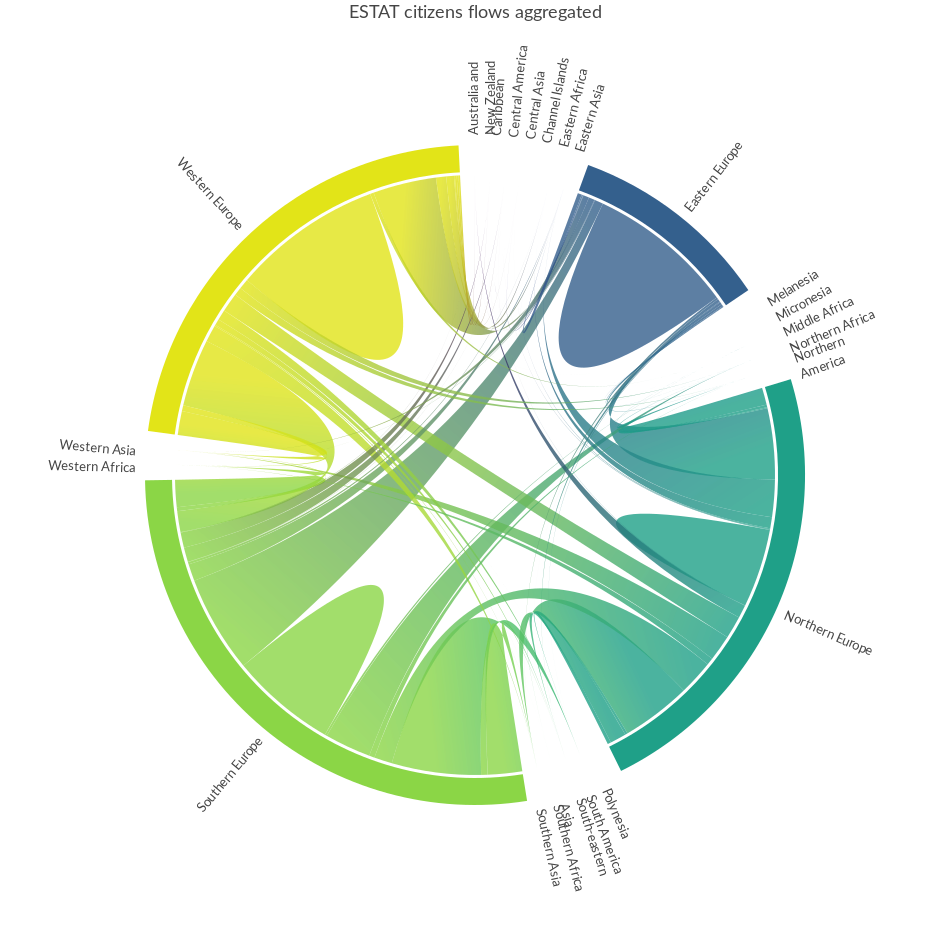
\includegraphics[width=1.0\textwidth]{images/ChordFlows/ESTAT_cit_True.png}
    \caption{Chordflow flussi cittadini ESTAT}
    \label{fig:chordestatcittrue}
\end{figure}
Questi grafici sono molto simili dato che quello di Crunchbase viene realizzato filtrando i dati analizzando solo quelli che sono presenti anche in ESTAT.\\ Verrà affrontato più in avanti un esempio di dati non filtrati Crunchbase per equità di analisi grafica. 

%%%%% RESIDENTI CONFRONTO ESTAT 

\begin{figure}[t]
    \centering
    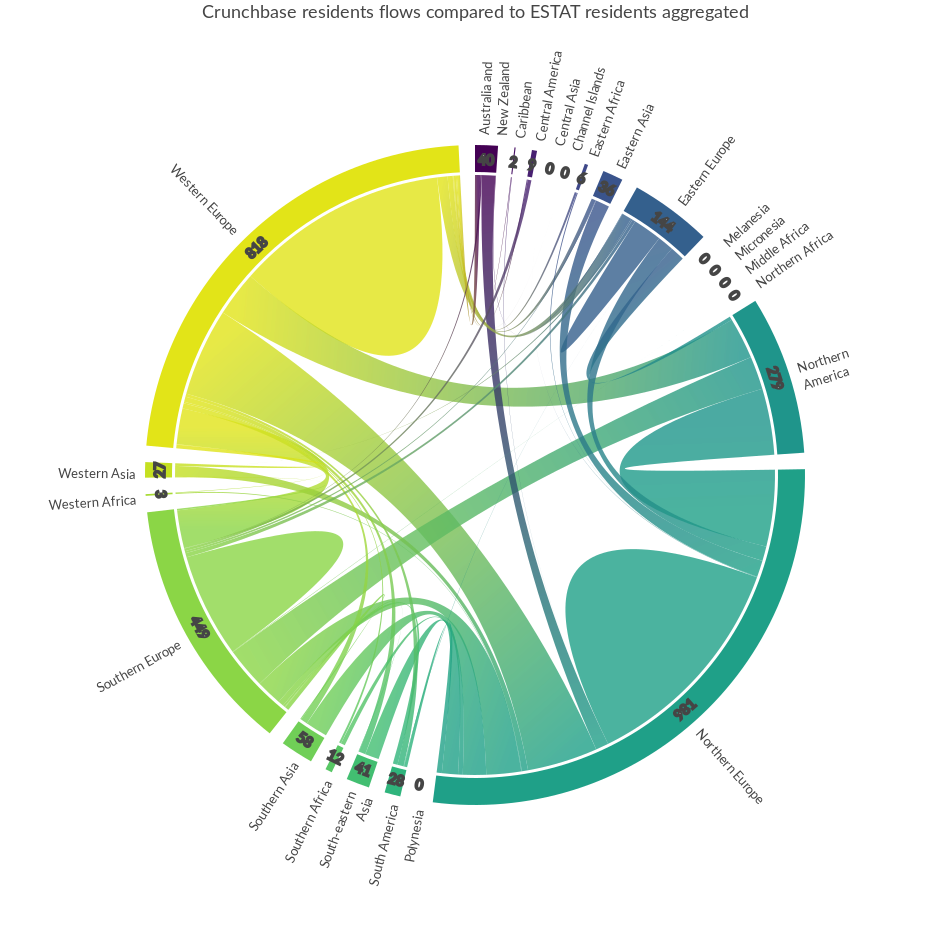
\includegraphics[width=1.0\textwidth]{images/ChordFlows/Crunchbase_res_ESTAT_True.png}
    \caption{Chordflow flussi Crunchbase in comparazione ai residenti ESTAT}
    \label{fig:chordcrunchestatrestrue}
\end{figure}
Potrebbe venire il dubbio che la figura \ref{fig:chordcrunchestatrestrue} relativa ai residenti sia identica alla figura \ref{fig:chordcrunchestatcittrue} relativa ai cittadini, ma per quanto simili differiscono leggermente. Questa discrepanza minima ci permette di assumere che la maggior parte delle persone che migrano per lavoro attraverso i dati ottenuti da Crunchbase, siano sia residenti che cittadini del paese di provenienza.
\begin{figure}[t]
    \centering
    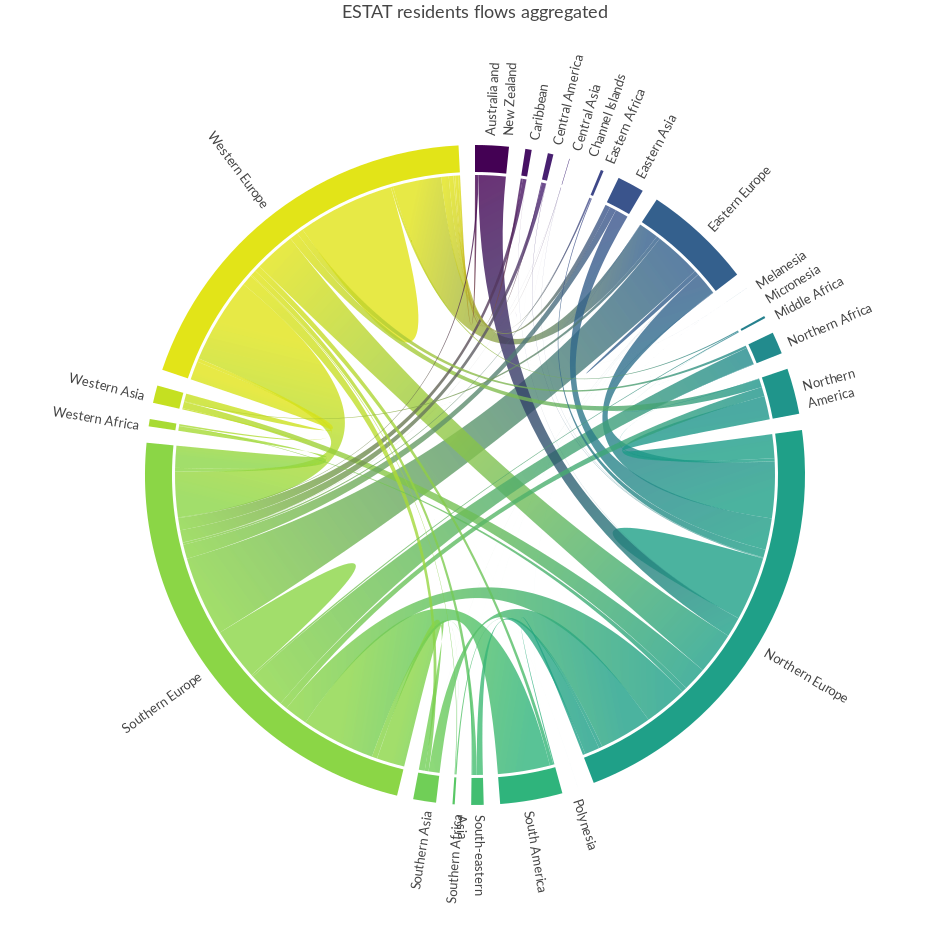
\includegraphics[width=1.0\textwidth]{images/ChordFlows/ESTAT_res_True.png}
    \caption{Chordflow flussi residenti ESTAT}
    \label{fig:chordestatrestrue}
\end{figure}
%Per 
Dai dati ESTAT possiamo vedere una differenza più importante per l'Est Europa rispetto ai flussi migratori dei cittadini della stessa zona. Nel grafico dei cittadini infatti la maggior parte dei flussi sono rientranti, abbiamo però che il chordflow di Crunchbase segue lo stesso modello.

%%%%% CITTADINI CONFRONTO UN 
\begin{figure}[t]
    \centering
    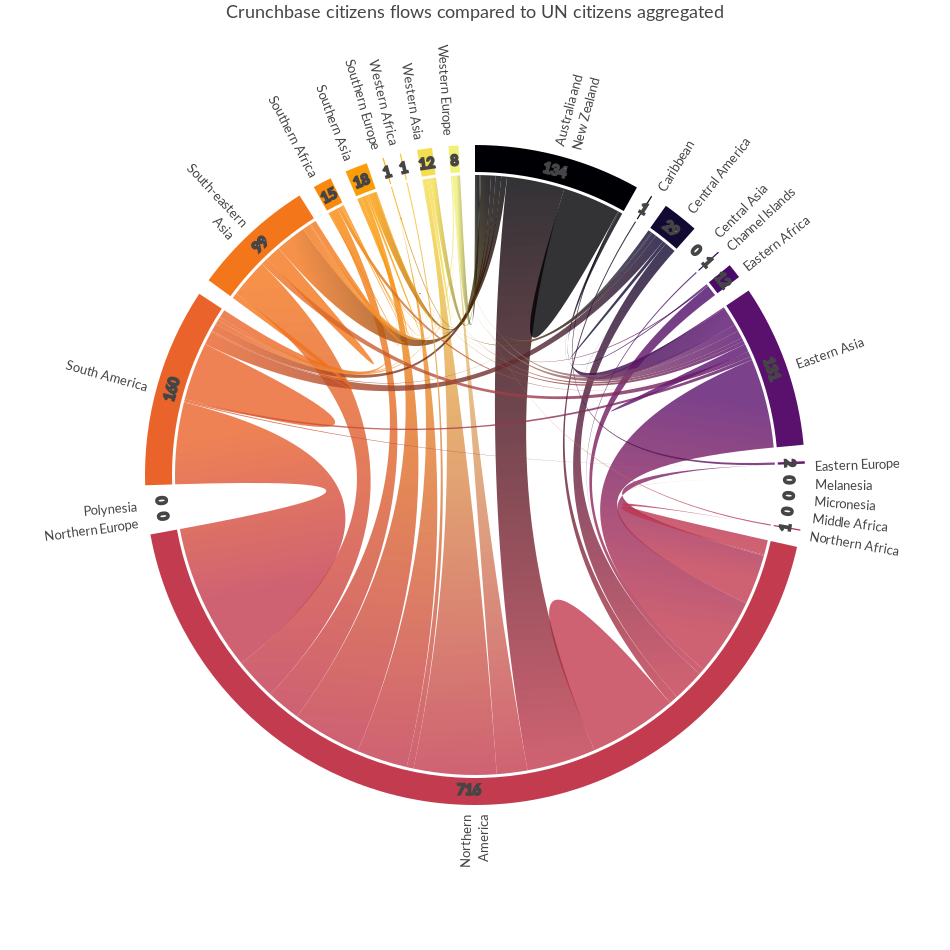
\includegraphics[width=1.0\textwidth]{images/ChordFlows/Crunchbase_cit_UN_True.png}
    \caption{Chordflow flussi Crunchbase in comparazione ai cittadini UN}
    \label{fig:chordcrunchuncittrue}
\end{figure}
%Come atteso 
I dati filtrati per comparazione ai dati UN sono più significativi per il continente nord americano. Il continente Europeo viene infatti in buona parte ignorato nei dati di United Nation, rendendo così difficile comparare i dati Crunchbase a dei dati reali veri e propri non essendo distribuiti in modo uniforme.
\begin{figure}[t]
    \centering
    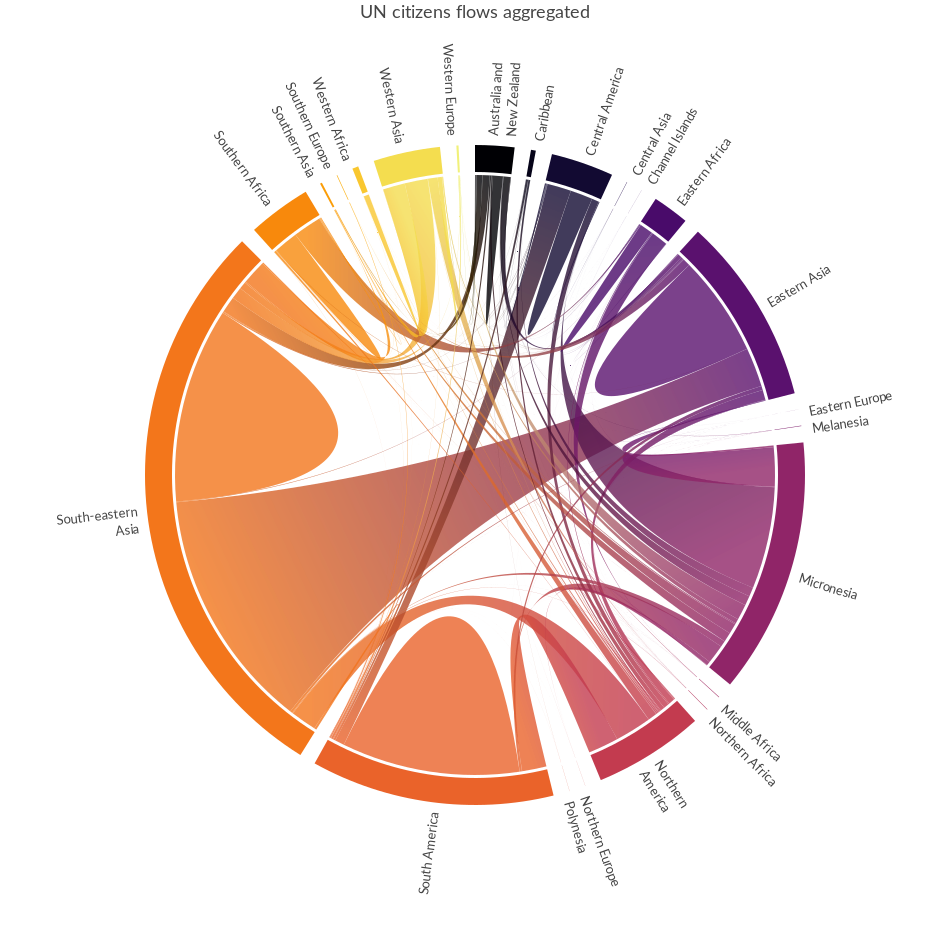
\includegraphics[width=1.0\textwidth]{images/ChordFlows/UN_cit_True.png}
    \caption{Chordflow flussi cittadini UN}
    \label{fig:chorduncittrue}
\end{figure}
%Come possiamo vedere i
Il grafico in Figura \ref{ } di Crunchbase comparato a quello di UN, seppur filtrato proprio attraverso i dati presenti nel dataset UN, non ha la stessa somiglianza che presentavano i grafici ESTAT. Questo può portare all'ipotesi che l'analisi dei dati attraverso Crunchbase sia più significativa per il continente Europeo ed il Nord America, non essendo di fatto presenti molti dati ad esempio sul sud-est asiatico come in UN.

%%%%% RESIDENTI CONFRONTO UN 

\begin{figure}[t]
    \centering
    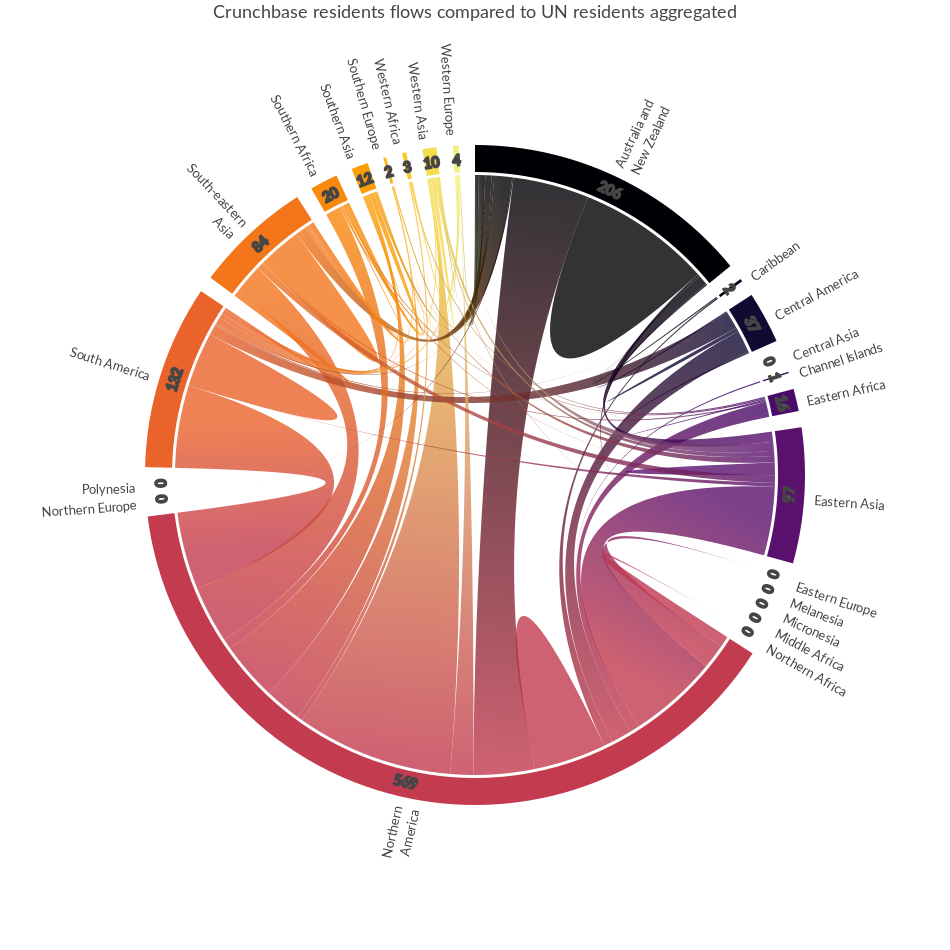
\includegraphics[width=1.0\textwidth]{images/ChordFlows/Crunchbase_res_UN_True.png}
    \caption{Chordflow flussi Crunchbase in comparazione ai residenti UN}
    \label{fig:chordcrunchunrestrue}
\end{figure}
%Come atteso il grafico relativo a
La Figura \ref{ } mostra i residenti di Crunchbase filtrati sugli stati in comune con UN.  è molto simile a quello dei cittadini. La differenza è minima questo porta in definitiva a definire Crunchbase rappresentante per il continente europeo e alcuni sub continenti particolari come il nord America o l'Oceania. 
\begin{figure}[t]
    \centering
    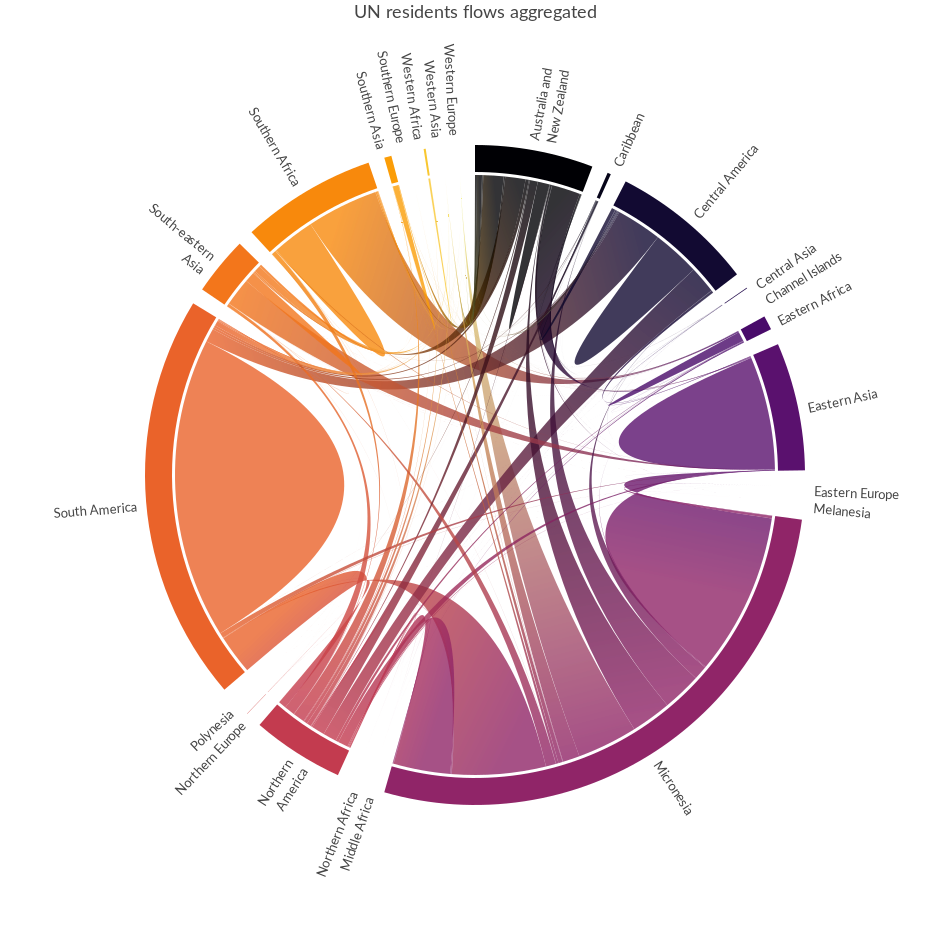
\includegraphics[width=1.0\textwidth]{images/ChordFlows/UN_res_True.png}
    \caption{Chordflow flussi residenti UN}
    \label{fig:chordunrestrue}
\end{figure}
%Vediamo come i 
I chordflow tra residenti e cittadini di UN sia molto differente, il che rende intuibile il perchè siano poco correlati i dati UN con quelli di Crunchbase che in genere si riferiscono in buona parte alle stesse persone quando facciamo la distinzione tra cittadini e residenti. 

%%%% CONFRONTO UN unito ESTAT

\subsubsection{ChordFlow Cittadini}
\begin{figure}[t]
    \centering
    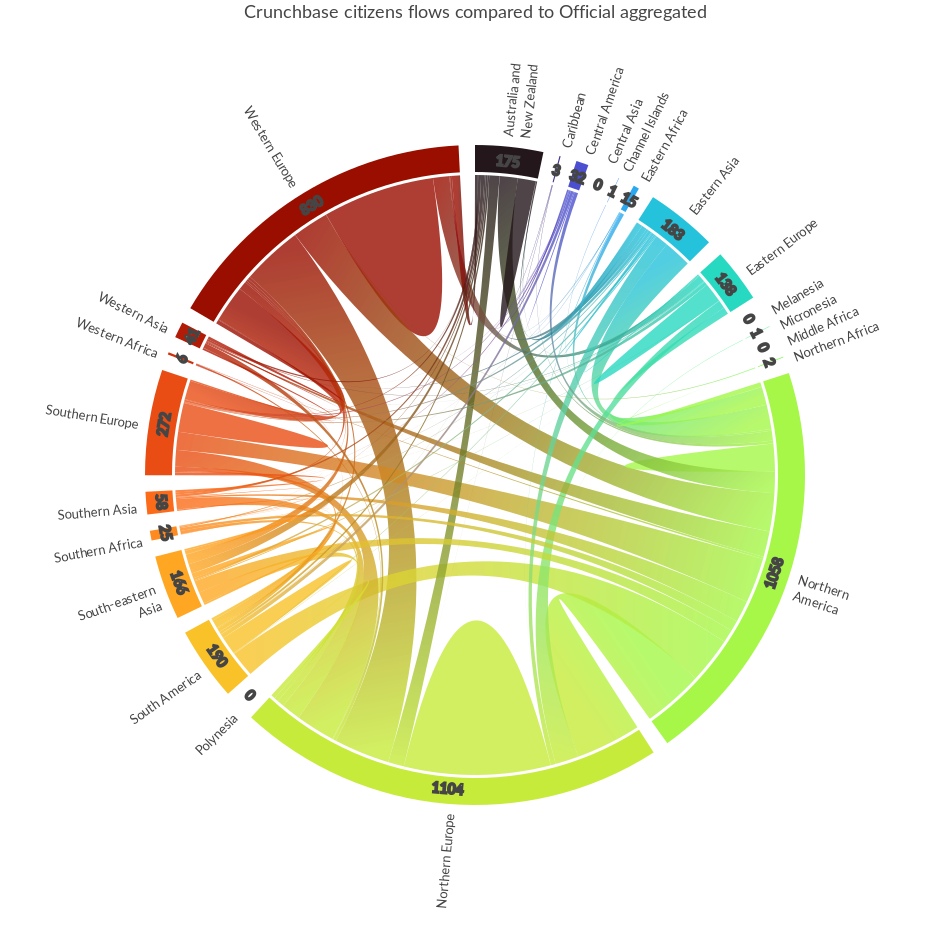
\includegraphics[width=0.8\textwidth]{images/congiunti/chords/Crunchabse_cit_off.png}
    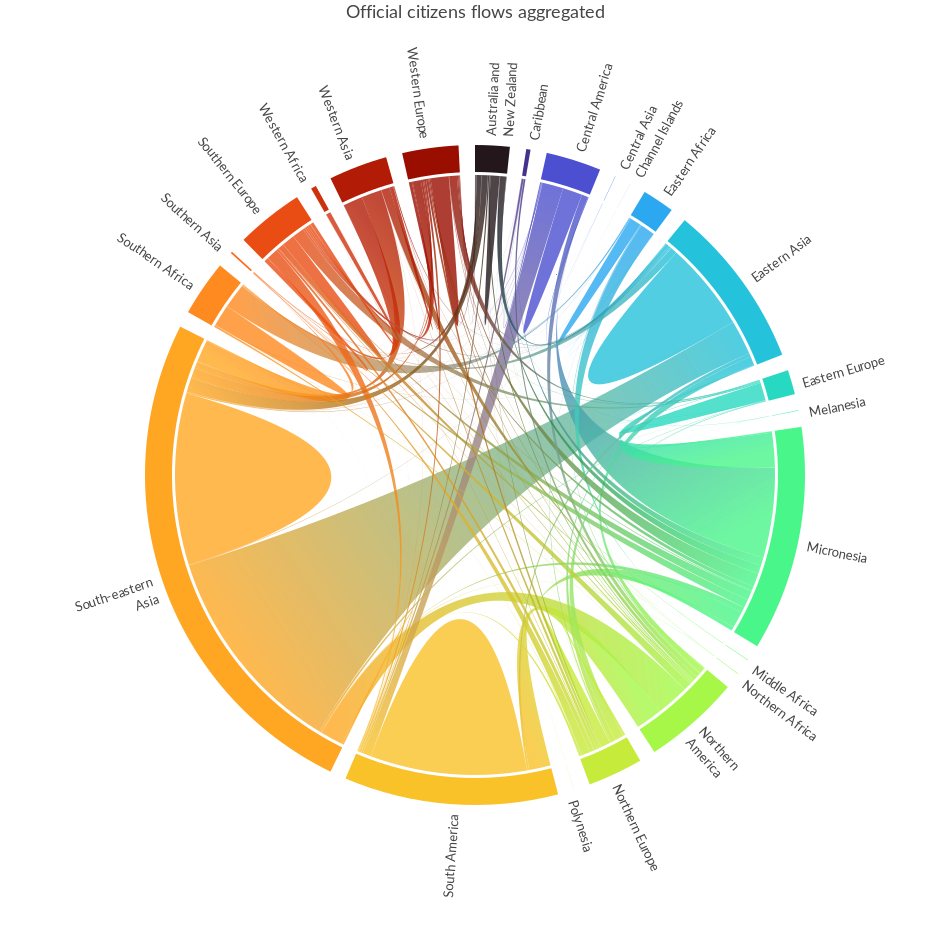
\includegraphics[width=0.8\textwidth]{images/congiunti/chords/Official_cit.png}
    \label{fig:chordoff_cit_true}
\end{figure}

\subsubsection{ChordFlow Residenti}
\begin{figure}[t]
    \centering
    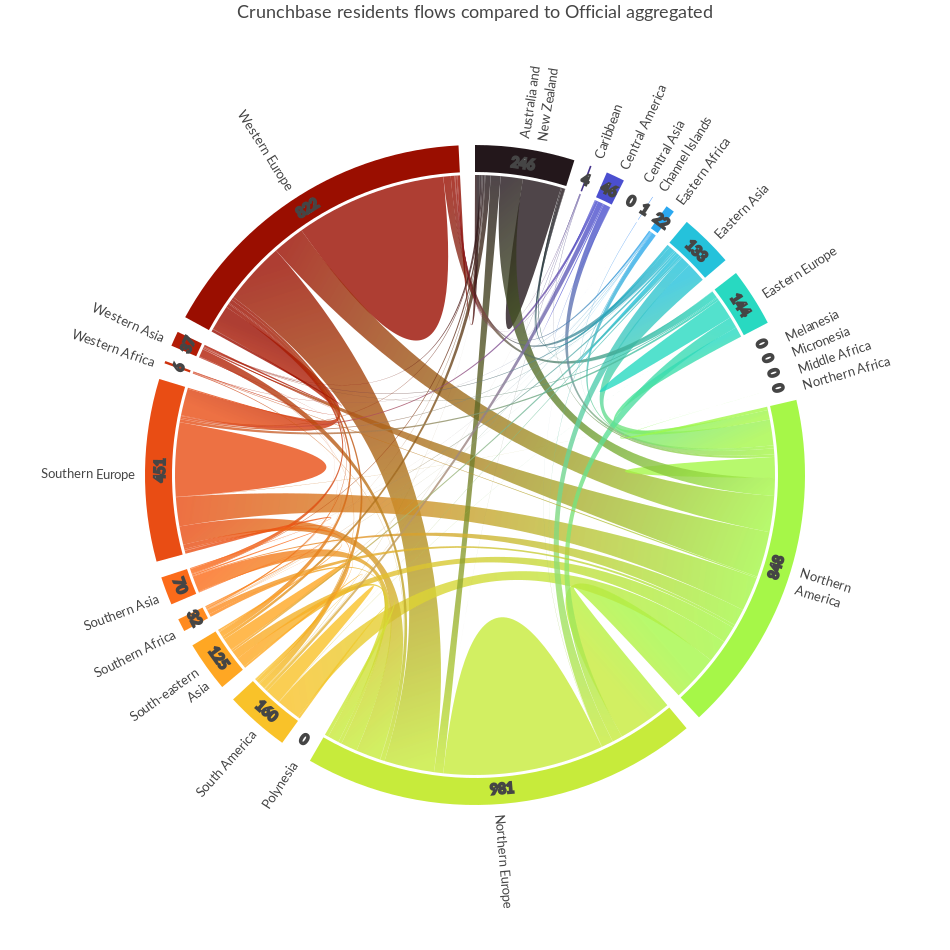
\includegraphics[width=0.8\textwidth]{images/congiunti/chords/Crunchabse_res_off.png}
    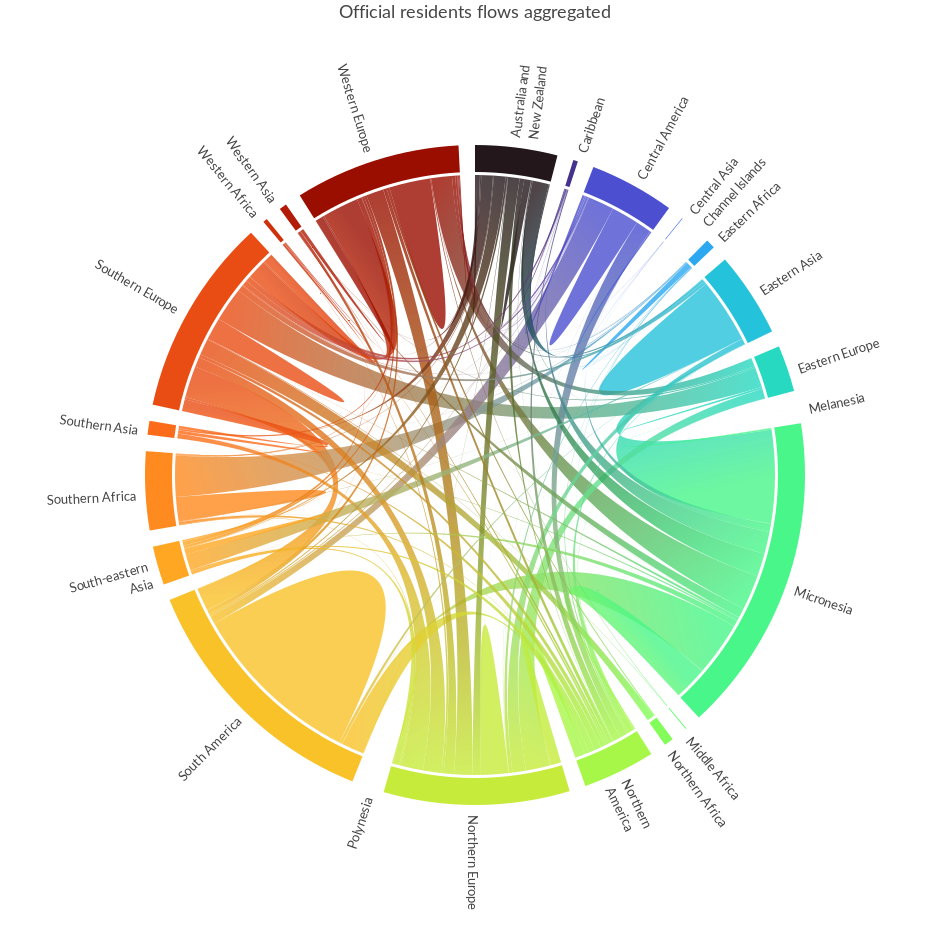
\includegraphics[width=0.8\textwidth]{images/congiunti/chords/Offcial_res.png}
    \label{fig:chordoff_res_true}
\end{figure}

%%%% FLUSSI CITTADINI E RESIDENTI ITALIANI ESTAT

\subsubsection{ChordFlow Cittadini Italiani}

\begin{figure}[t]
    \centering
    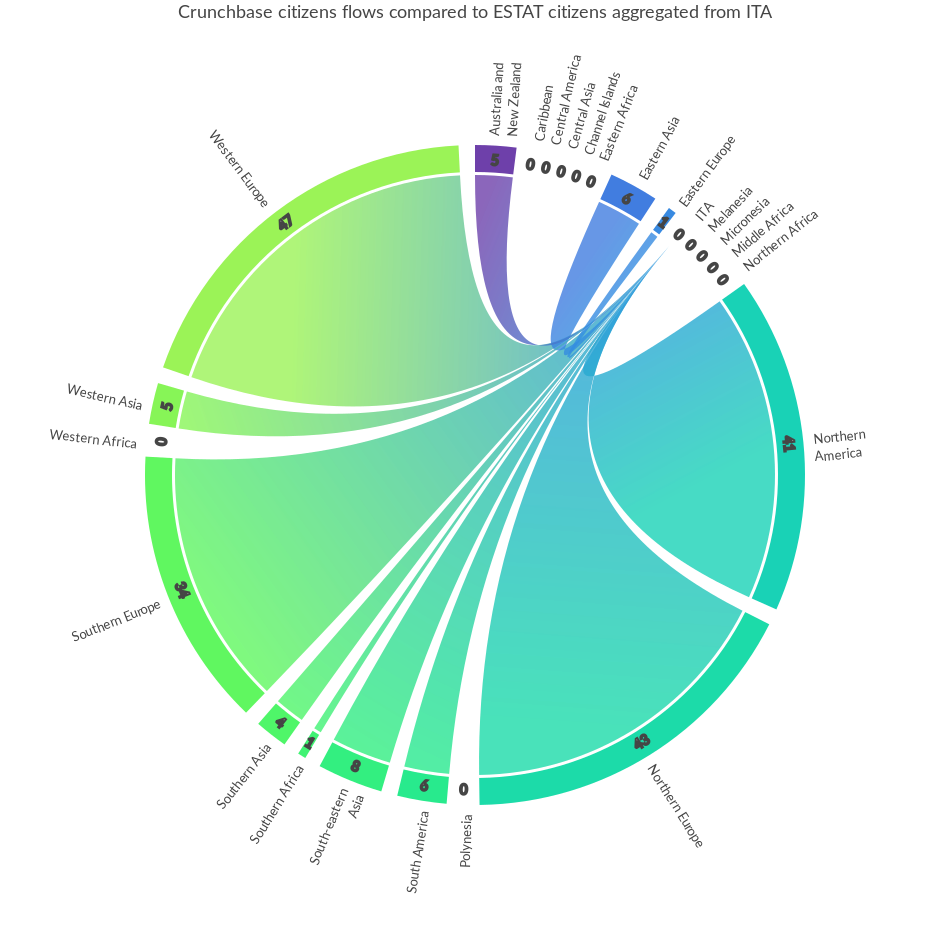
\includegraphics[width=0.8\textwidth]{images/ChordFlows/filtered_nationality/ita/Crunchbase_cit_ESTAT_True.png}
    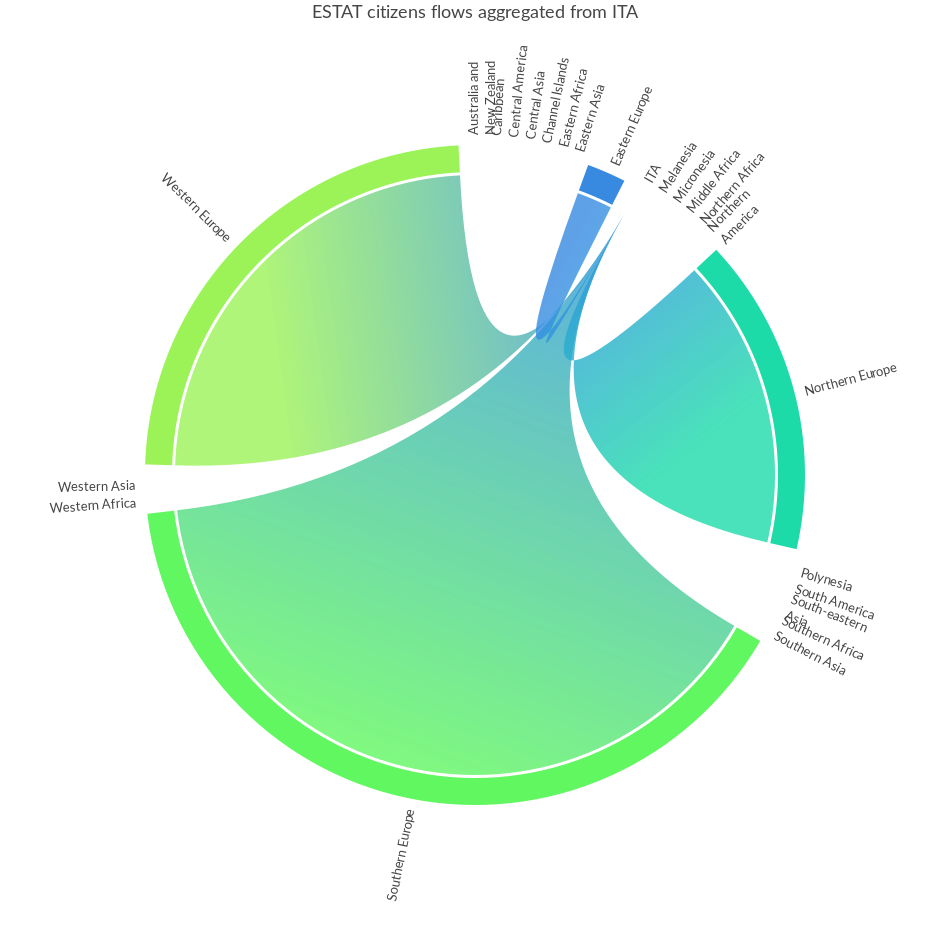
\includegraphics[width=0.8\textwidth]{images/ChordFlows/filtered_nationality/ita/ESTAT_cit_True.png}
    \label{fig:chordita_nat_true}
\end{figure}
\subsubsection{ChordFlow Residenti Italiani}
\begin{figure}[t]
    \centering
    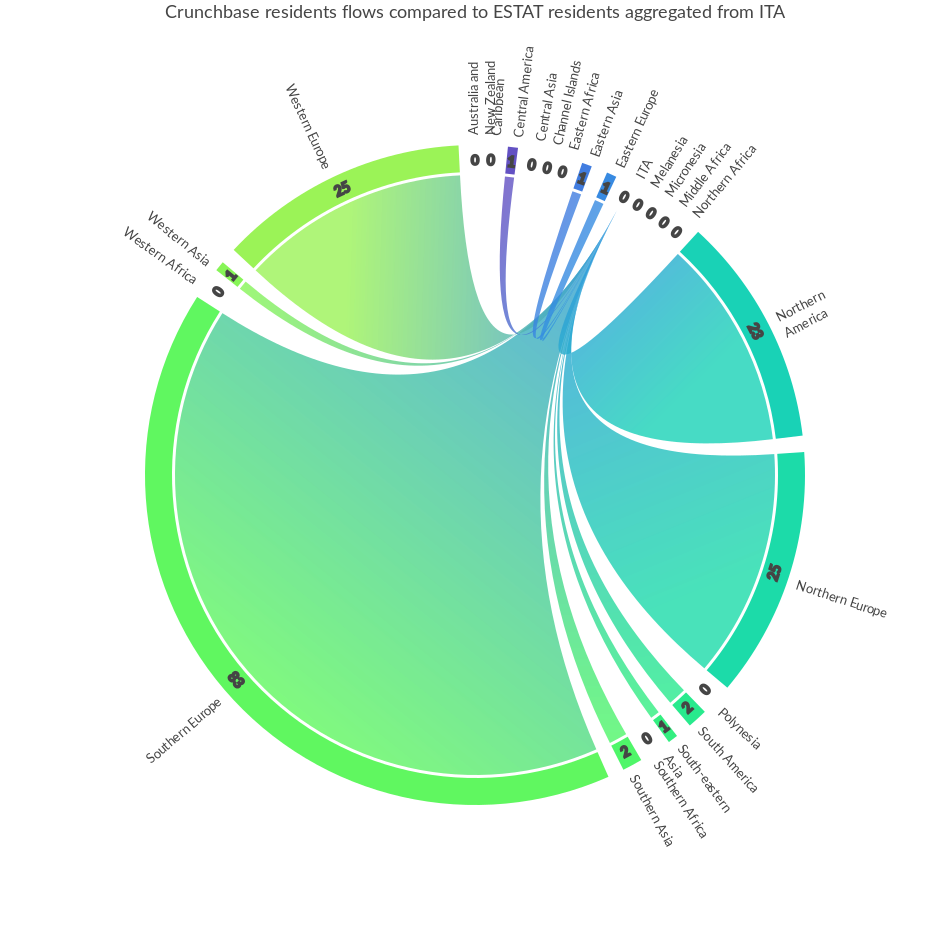
\includegraphics[width=0.8\textwidth]{images/ChordFlows/filtered_nationality/ita/Crunchbase_res_ESTAT_True.png}
    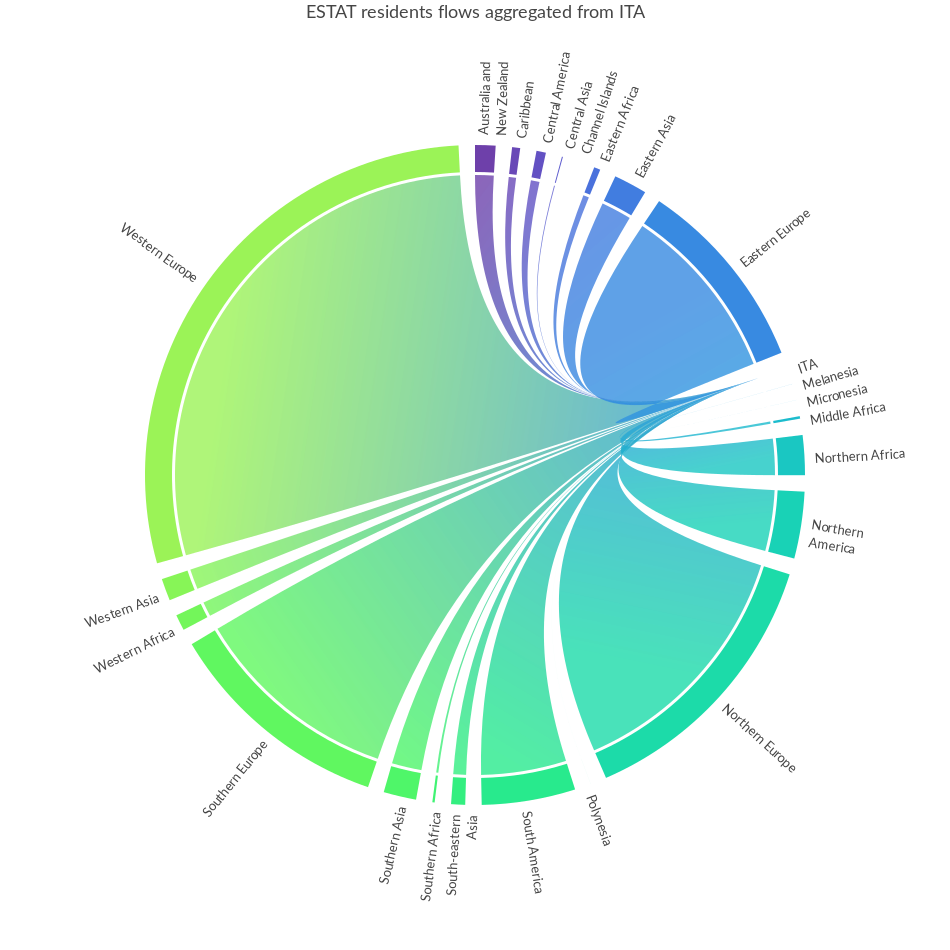
\includegraphics[width=0.8\textwidth]{images/ChordFlows/filtered_nationality/ita/ESTAT_res_True.png}
    \label{fig:chordita_res_true}
\end{figure}

%%%% FLUSSI IMMIGRAZIONE IN ITALIA ESTAT

\subsubsection{ChordFlow Cittadini Esteri Migrati In Italia}
\begin{figure}[t]
    \centering
    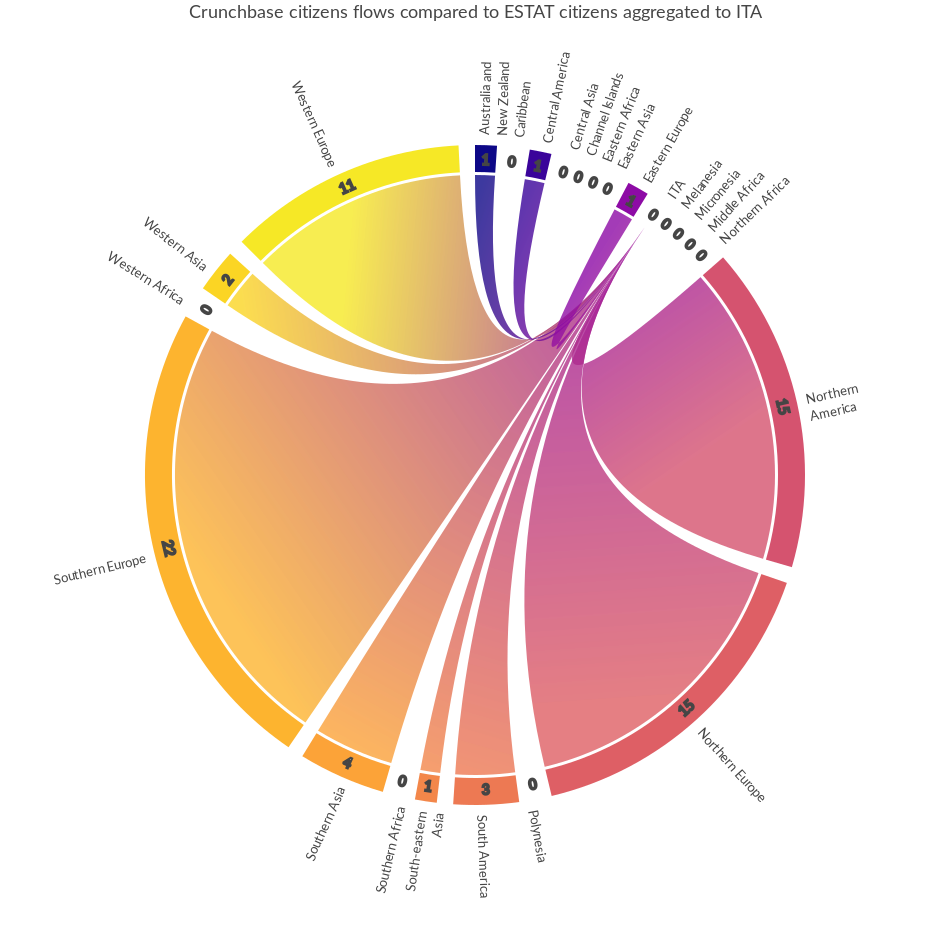
\includegraphics[width=0.8\textwidth]{images/ChordFlows/filtered_destination/ita/Crunchbase_cit_ESTAT_True.png}
    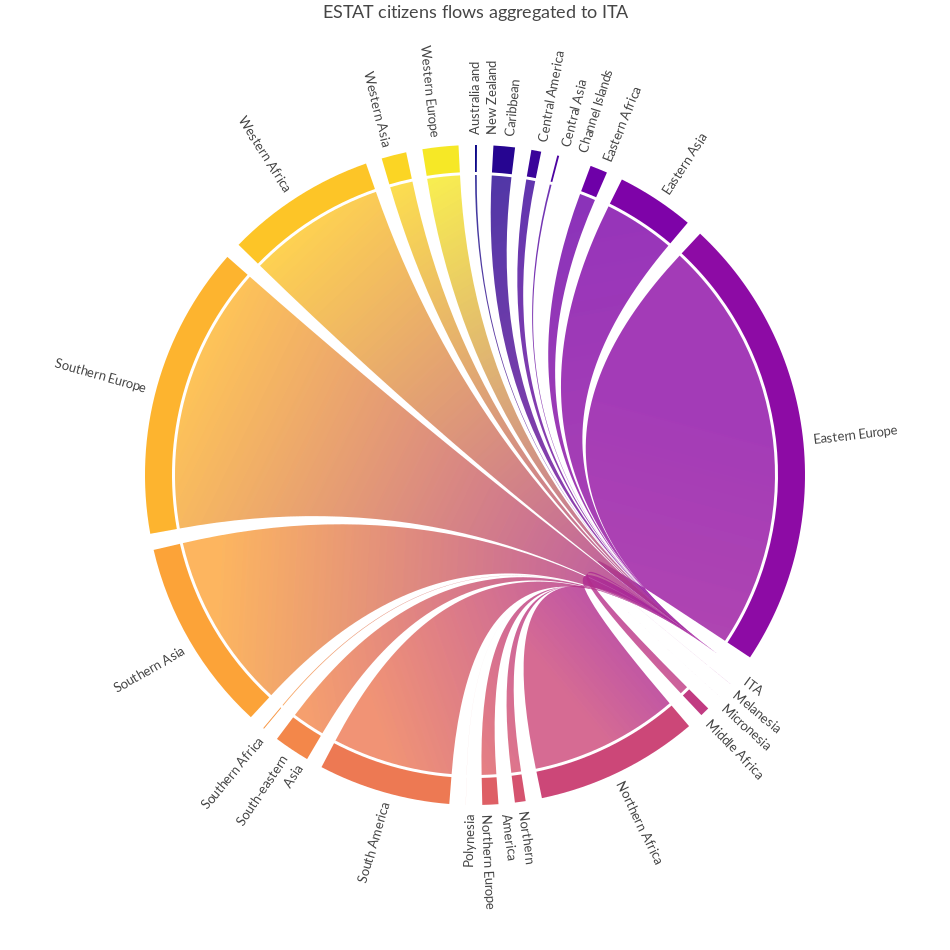
\includegraphics[width=0.8\textwidth]{images/ChordFlows/filtered_destination/ita/ESTAT_cit_True.png}
    \label{fig:chordtoita_nat_true}
\end{figure}
\subsubsection{ChordFlow Residenti all'Estero Migrati In Italia}
\begin{figure}[H]
    \centering
    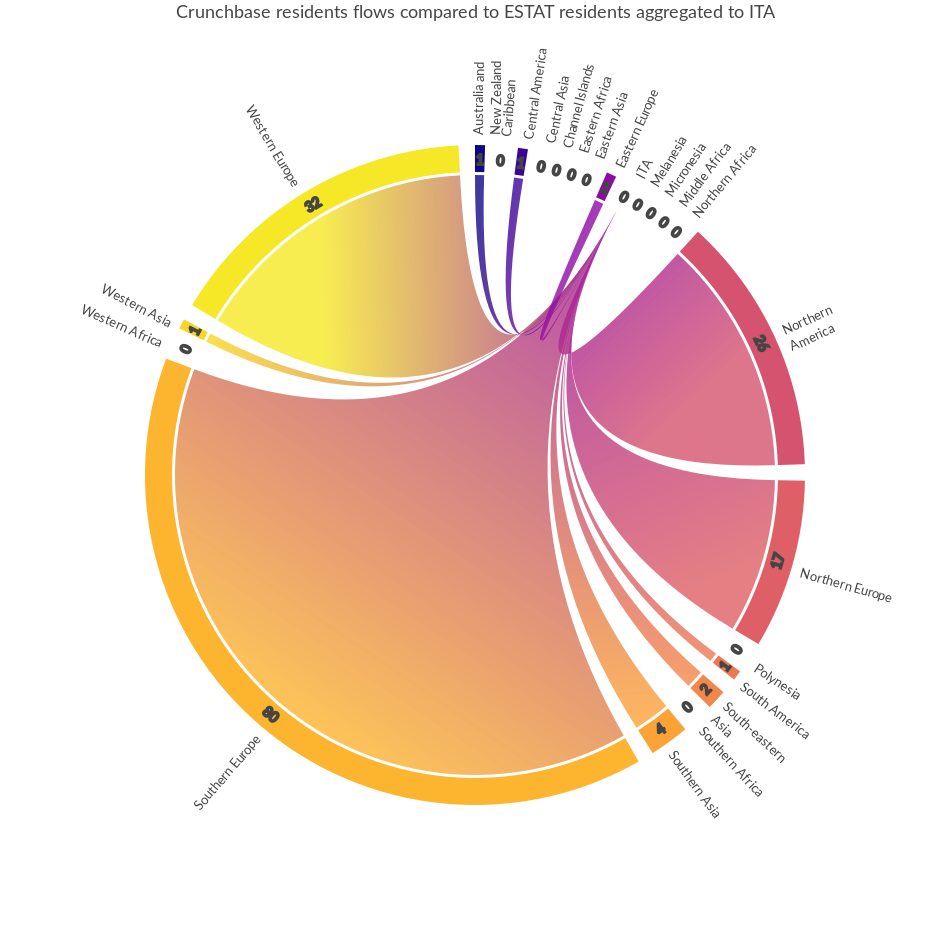
\includegraphics[width=0.8\textwidth]{images/ChordFlows/filtered_destination/ita/Crunchbase_res_ESTAT_True.png}
    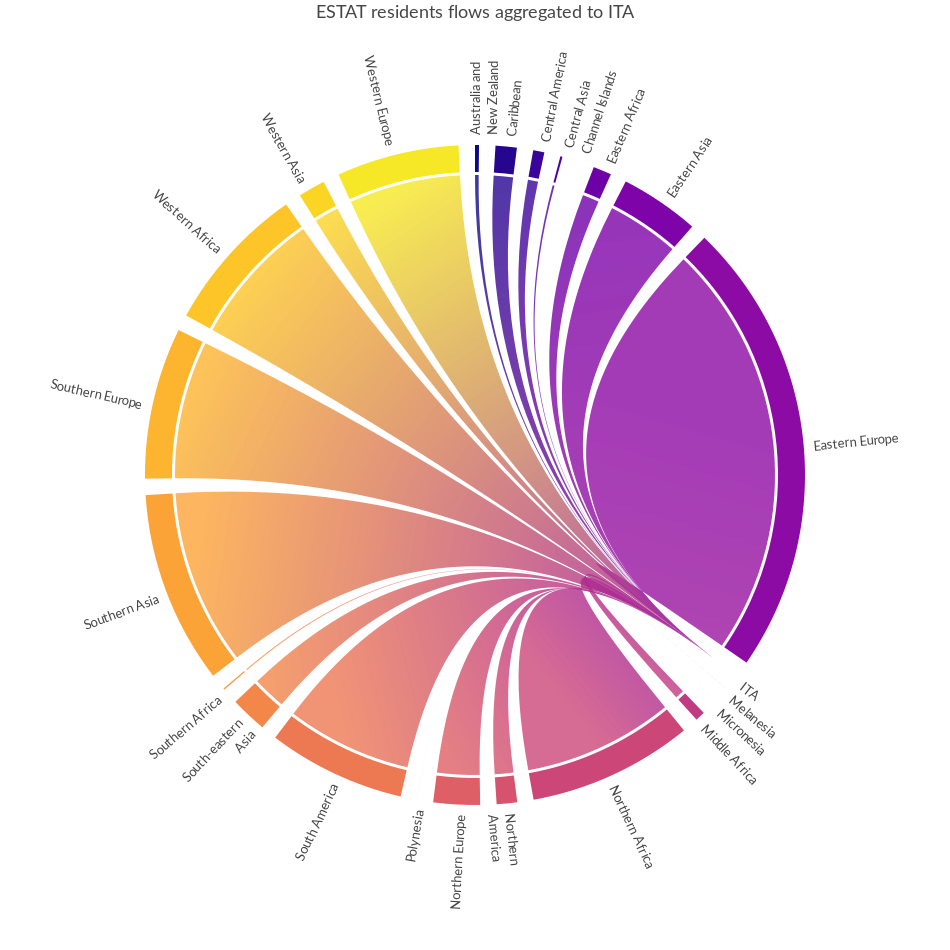
\includegraphics[width=0.8\textwidth]{images/ChordFlows/filtered_destination/ita/ESTAT_res_True.png}
    \label{fig:chordtoita_res_true}
\end{figure}

%%%% FLUSSI CITTADINI E RESIDENTI INGLESI ESTAT

\subsubsection{ChordFlow Cittadini UK Che Emigrano all'Estero}
\begin{figure}[t]
    \centering
    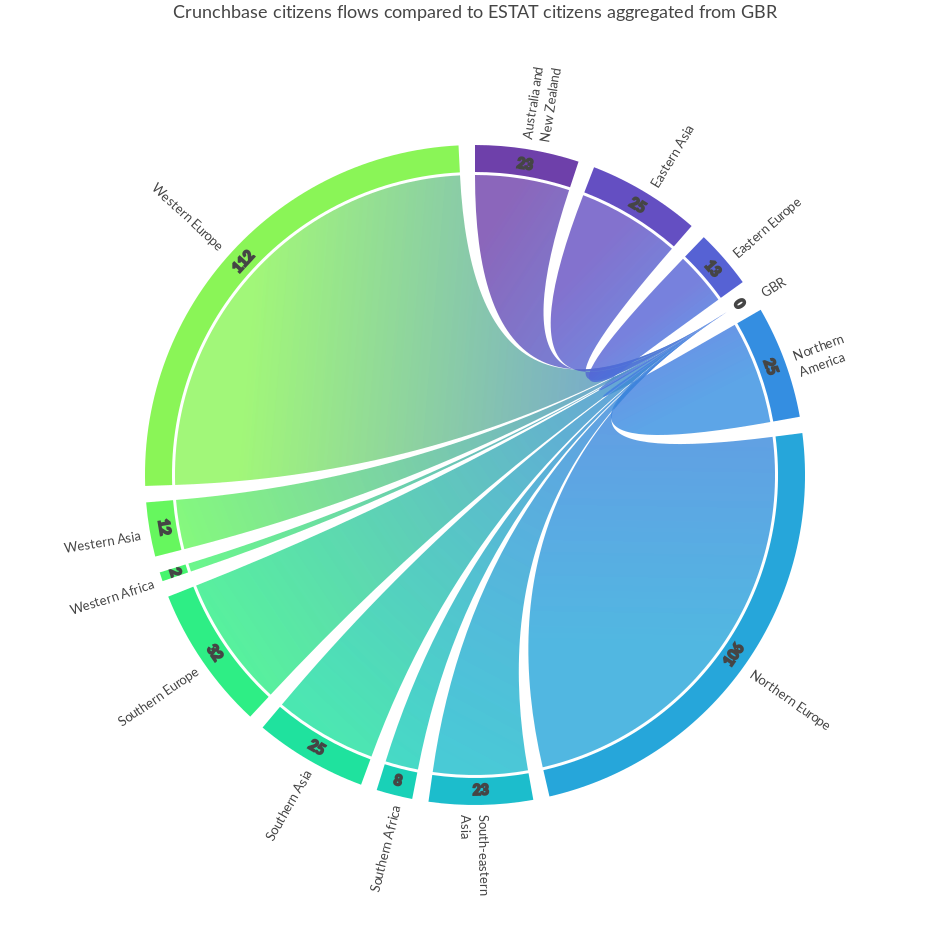
\includegraphics[width=0.8\textwidth]{images/ChordFlows/filtered_nationality/gbr/Crunchbase_cit_ESTAT_True.png}
    \includesvg[inkscapelatex=false, width=0.75\textwidth]{Chords/filter_estat_gbr/GBRESTAT_CIT}
    \label{fig:chordgbr_cit_true}
\end{figure}
\subsubsection{ChordFlow Residenti in UK Che Emigrano all'Estero}
\begin{figure}[t]
    \centering
    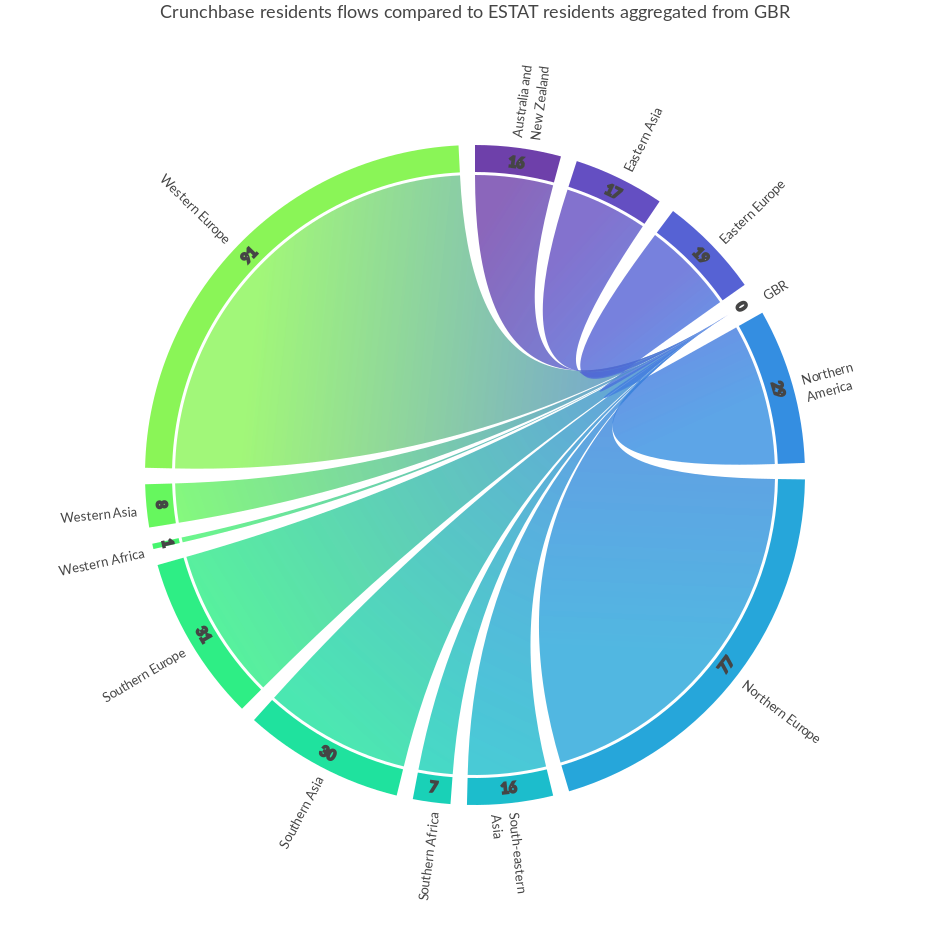
\includegraphics[width=0.8\textwidth]{images/ChordFlows/filtered_nationality/gbr/Crunchbase_res_ESTAT_True.png}
    \includesvg[inkscapelatex=false, width=0.75\textwidth]{Chords/filter_estat_gbr/GBRESTAT_RES}
    \label{fig:chordgbr_res_true}
\end{figure}

%%%% FLUSSI IMMIGRAZIONE IN INGHILTERRA ESTAT
\subsubsection{ChordFlow Cittadini Esteri Migrati In UK}
\begin{figure}[H]
    \centering
    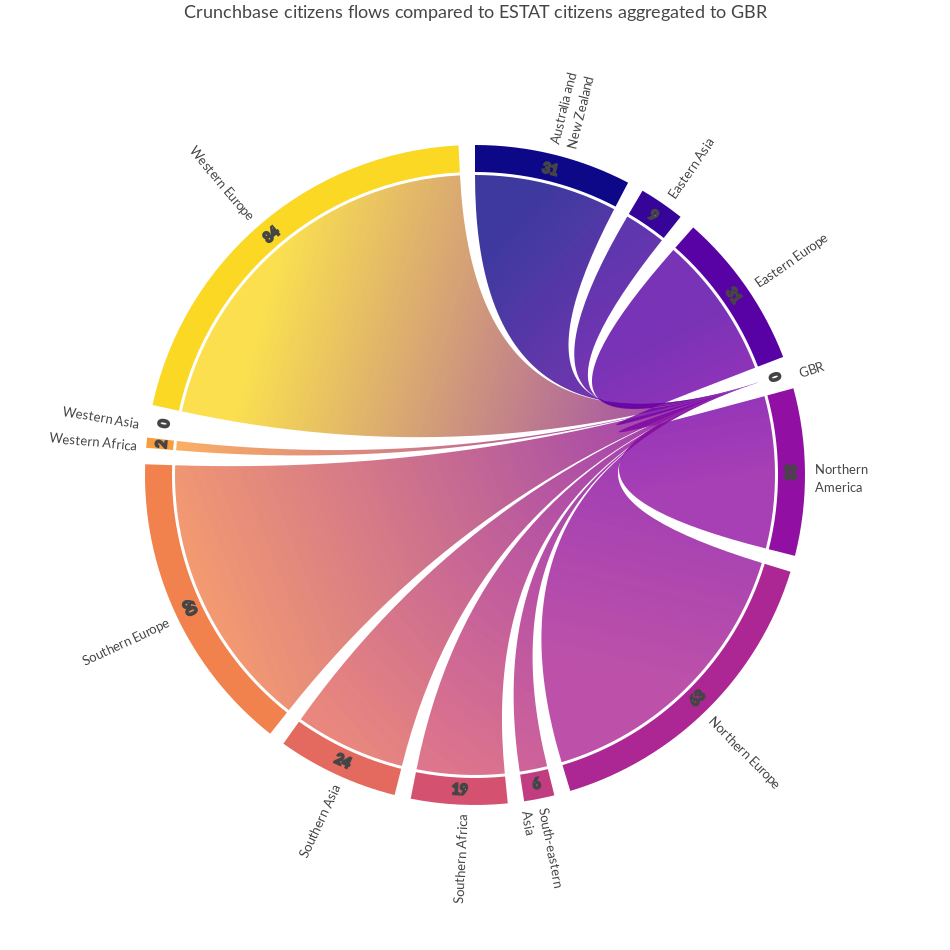
\includegraphics[width=0.8\textwidth]{images/ChordFlows/filtered_destination/gbr/Crunchbase_cit_ESTAT_True.png}
    \includesvg[inkscapelatex=false, width=0.75\textwidth]{Chords/filter_estat_gbr/TOGBRESTAT_CIT}
    \label{fig:chordtogbr_cit_true}
\end{figure}
\subsubsection{ChordFlow Residenti all'Estero Migrati In UK}
\begin{figure}[H]
    \centering
    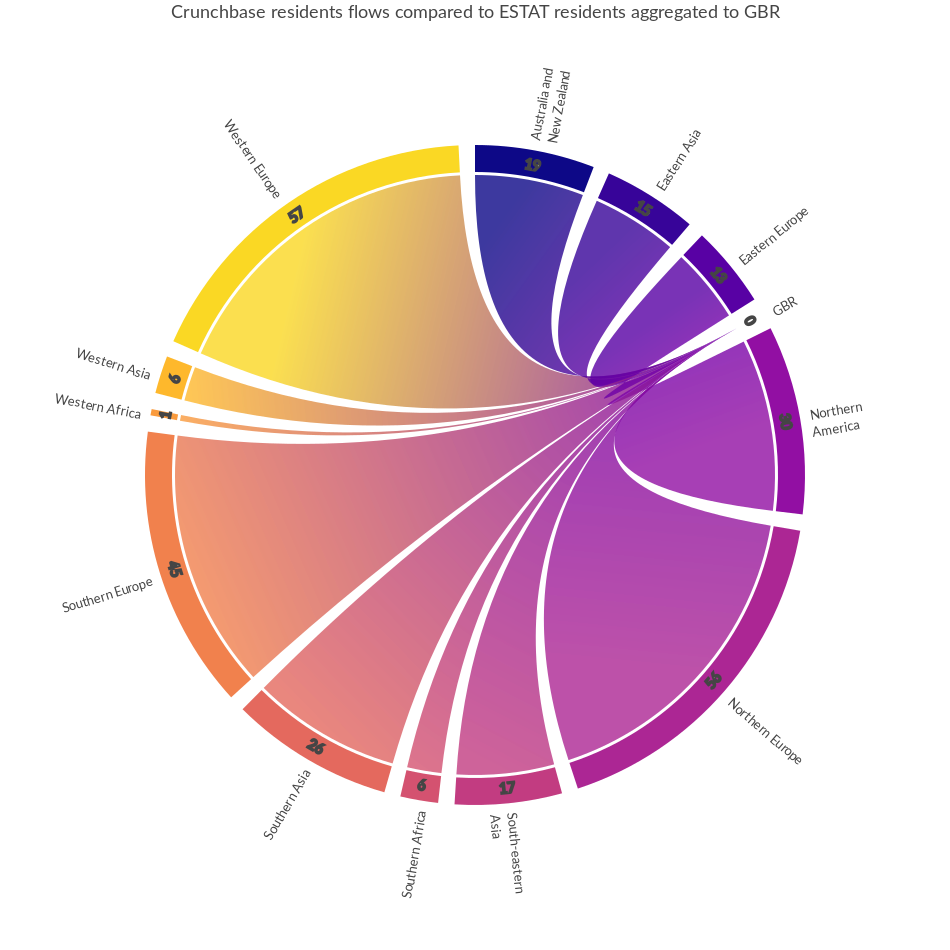
\includegraphics[width=0.8\textwidth]{images/ChordFlows/filtered_destination/gbr/Crunchbase_res_ESTAT_True.png}
    \includesvg[inkscapelatex=false, width=0.75\textwidth]{Chords/filter_estat_gbr/TOGBRESTAT_RES}
    \label{fig:chordtogbr_res_true}
\end{figure}